\RequirePackage[T1]{fontenc}
\documentclass[conference]{IEEEtran}
\usepackage{amsmath,amssymb,graphicx,booktabs,array,url}
\usepackage[hidelinks]{hyperref}
\newcolumntype{P}[1]{>{\raggedright\arraybackslash}p{#1}}
\newcommand{\degc}{^{\circ}}
\newcommand{\asset}[2]{\IfFileExists{#1}{\includegraphics[width=\columnwidth]{#1}}{\fbox{\parbox[c][25mm][c]{0.92\columnwidth}{\centering #2\\Illustrative figure pending export}}}}
\newcommand{\shot}[2]{\fbox{\parbox[c][28mm][c]{0.92\columnwidth}{\centering\textbf{App screenshot placeholder #1}\\#2\\No device capture supplied.}}}

\title{Visual Privacy on Smartphones Based on Context: Adaptive Protection and Undetectable but Readable Areas}
\author{\IEEEauthorblockN{Author particulars still pending}\IEEEauthorblockA{Prototype of a university project\\Organisation and contact information still to be determined}}

\begin{document}
\maketitle

\begin{abstract}
An viewer can use the front-camera detection zone to read a smartphone outside. This article examines residual exposure using a Flutter privacy prototype and a geometrical comparison of three different techniques: a privacy-screen protector, a clip-on fisheye, and an outside human-tracking radar. Local face counting, orientation sensing, and a session-only AES-256-GCM vault are all combined in the program. The baseline is expanded by an Android-local embedding verifier, PIN fallback, and reauthorization latch; physical validation remains pending.

The readable but undetected area consists of readable places outside of effective sensing coverage. Analytical widths are determined at 35, 40, 55, and 60 cm utilizing clearly assumed scenario angles of 75 degrees for the camera, 60 degrees for filter readability, and 120 degrees for useful fisheye coverage. The camera and filtered readable widths are 61.39 and 46.19 cm at 40 cm, respectively. Their perfect aligned containment does not indicate body occlusion protection.

A different simulator shows every six sensor/filter combinations. There is no physical calibration data set, recognition benchmark, or measured exposure latency; numerical results are based on geometric calculations instead of device measurements. A fillable data schema and calibration method help with later empirical analysis.
\end{abstract}

\begin{IEEEkeywords}
visual privacy, shoulder surfing, AES-GCM, face verification, privacy filter, radar, fisheye
\end{IEEEkeywords}

\section{Intro}
Sensitive words and images show up when a real user looks at them. Stored bytes cannot be encrypted to stop a viewer from reading the shown pixels. The setting of shoulder surfing also matters: Abdrabou et al. investigate opportunistic observation in public transportation using mobile eye tracking and point out the technical challenge of observing it in natural environments~\cite{Abdrabou2025Shoulder}. A privacy device so has to have a rendering policy and an account of where an viewer may stay unobserved.

The motivating prototype tracks device orientation and utilizes the front camera to spot faces. The project owner claims the phone has a privacy-screen protector and that the main physical setup intended is the protector-plus-app combination. Neither the fitted filter nor the camera has an appropriate calibration record. We therefore provide a scenario analysis and software review rather than a finished actual experiment.

The contribution is a typical geometric goal, the readable-but-undetected region, therefore connecting the program to three sensing/filter techniques. We calculate finite-plane widths, differentiate between optical specifications and practical detection angles, and create radar counting without giving radar targets identity. We also outline repeatable calibration and authentication assessment methods. The numerical tables are derived from provided reference ranges and explicit assumptions; they should not be seen as actual accuracy or a privacy statement.

\section{Related Work and Sorce Scope}
For mobile devices, \emph{iScreen} is a commercial software-based screen-privacy technology~\cite{Lei2021iScreen}. From the minutes record, its title, writers, location, pages, and DOI are clearly visible; we make no comparative latency or accuracy claim without checking its whole method. Though they don't calibrate the device used here, Abdrabou et al.~\cite{Abdrabou2025Shoulder} inspire study of natural observer behavior.

Huo and others look at an image-encryption structure using a three-dimensional hyperchaotic system~\cite{Huo2025AES}. This repository does not include that structure; this prototype employs the conventional AES-GCM interface. Rather than a claimed performance transfer from an image-encryption study, NIST's GCM recommendation is the relevant cryptographical design reference~\cite{NISTGCM}. Liu et al.~\cite{Liu2025Monocular} present a monocular depth-estimation network. Though neither owner verification nor a component used here, depth estimate may help with future spatial thinking. ML Kit clearly divides face identification from recognition~\cite{MLKit}; a face count by itself cannot identify the owner.

Wide-angle optics call for an appropriate projection and calibration model. Kannala and Brandt~\cite{Kannala2006} go through designs for fisheye, wide-angle, and traditional lenses. Manufacturer manuals set a nominal angle for an example clip-on~\cite{Kenko}; radar documentation sets module-level operating conditions~\cite{LD2450,LDProtocol}. Our suggested phone setup sets neither detection dependability.

The project owner provided two more works: Zeeshan, Moradpoor, and La Spada's \emph{Observer-Aware Runtime Exposure Mitigation for Mobile Edge Devices}, marked SafeComp 2026/Research Gate 406502212, and Prasad's \emph{From Screen Exposure to Street-Level Risk}, tagged 2026/Research Gate 404821939, DOI 10.13140/RG.2.2.22618.30400. Not separately checked were complete authoritative publication metadata and content. A different given bibliography holds them, therefore they do not back up factual claims in this article.

\section{Threat Models and Objectives}
The owner looks at graphic material on an uncompromised phone. A third party may stand sideways, behind the owner, or outside the range of the selfie camera. Direct visual exposure is under consideration; outside the assessed model are remote compromise, forensic extraction, reflection attacks, telephoto recording, and an attacker regulating the sensor feed. Still a clear restriction rather than a recognized defense is authentication spoofing.

Let $R(t)$ be spots from which material is readable at time $t$, and let $D_c(t)$ be places the camera can truly see an viewer. Specify:
\begin{equation}
 B(t)=R(t)\setminus D(t).
 \label{eq:blind}
\end{equation}
where for optical-only running $D=D_c$. For an ideal autonomous presence sensor, spatial coverage is described by $D_c\cup D_r$; nonetheless, radar count-based policies call for more nuance: a reported radar target is not always enough to trigger defense. Therefore, we also define $B_{\rm policy}$ as observable locations where the ultimate threat rule stays false. If radar only detects the observer and misses the owner, its count might be one; that observer is outside the coverage of the policy even if they are inside $D_r$.

Range, lighting, posture, occlusion, and detector confidence all affect coverage. A geometric sector gives an upper limit on maybe useable sensing places. For a finite evaluation area $\Omega$, $|B\cap\Omega|/|R\cap\Omega|$ is a possible area-based exposure metric when the denominator is nonzero; it is not an assault probability. The current work gives widths and samples instead of estimating this measure from human tests.

\section{Foundational Programme and Authentication Agreement}
\subsection{Verified Installation}
With native-mobile ML Kit face recognition, the repository employs Flutter. The examined camera monitor selects the front camera, asks for medium resolution, turns off audio, utilizes rapid detection with minimum facial size of 0.08, and throttles processing to at most one frame per 200 ms. These are code configurations rather than measured throughput. To safeguard information, detection mistakes, app inactivity, and a three-second stale-data timeout help to Android's orientation derives from a platform event channel's game rotation vector. Device-dependent orientation thresholds call for independent calibration.

The checked Content Vault generates an AES-256-GCM session key, seals every item with its identifier as linked data, and shows only decrypted clear buffers. A revision counter helps to lock drops application references to clear material and invalidates in-flight decryption. This does not prove safe managed memory, GPU textures, or decoded image cache erasure. Though not encrypted asset distribution, bundled demonstration assets are still available in the application package. The session key stays in process memory.

The baseline face controller normally restored material after three frames and at most one face. The present version authenticates and a constant reauthorization requirement replaces count-only restoration. Mobile FaceNet with ML Kit landmarks and tracking is utilized on Android; desktop and web maintain count-based detecting and PIN fallback. Below are execution specifics derived from source analysis and the integration report rather from physical Android validation. For this deliverable, no Android smartphone was connected:

\begin{table}[t]\caption{Evidence boundary for the application.}\label{tab:status}\centering\footnotesize
\begin{tabular}{@{}P{0.39\columnwidth}P{0.52\columnwidth}@{}}\toprule
Component & Evidence/status\\\midrule
Local face count, orientation stream & Present in inspected source; device performance unmeasured\\
AES-256-GCM session vault & Present; no claim of whole-device protection\\
Privacy protector & Owner-reported installed; uncalibrated\\
Owner embeddings, PIN, persistent latch & Implemented extension; physical validation pending\\
Fisheye and external radar & Proposed/modelled; no phone integration established\\\bottomrule
\end{tabular}\end{table}

\begin{figure}[t]\centering
\asset{figures/architecture.pdf}{Camera and orientation $\rightarrow$ policy $\rightarrow$ pixel gate and AES vault; authentication authorizes restoration; radar is proposed.}
\caption{Architecture and evidence boundaries. Authentication is an implemented extension awaiting physical validation; radar remains proposed.}\label{fig:arch}\end{figure}

\subsection{Required Reauthorization State Machine}
The extension separates approved display, threat detected, safeguarded content, and reauthentication required. Sensitive widgets are gated when authentication or the vault is locked. A state update causes Flutter rebuilding: obscuration goes on for the following paint, not in sync with the sensor callback. Asynchronous encryption by itself cannot stop a frame that has already been shown; the first totally hidden frame's delay is unknown.

Once protected, an extra observer's disappearance does not automatically allow access. Appropriate PIN entry or three allowed face results will help to reauthorize following physical sensing clearance. Unsuccessful PIN tries still locked. For a continuously monitored single face, a PIN-approved session may handle inadequate identification data but not numerous faces, bad orientation, or camera malfunction; tracking/count updates negate this exclusion. This clear fallback strategy is less effective than continuous biometric identification assurance.

The Android verifier employs a Mobile FaceNet model with 192-dimensional output and 112 by 112 RGB input. Chen et al. provide the main architectural reference~\cite{MobileFaceNets}; their reported performance is not a benchmark for this software or these weights. Enabled are ML Kit benchmarks and monitoring. Two-eye alignment causes ambiguity when NV21 frames are supported; clipping, inadequate size, great posture, incorrect exposure, or unsupported layout.

Eight samples separated by at least 400 ms are needed for enrolment; reference comes from normalised embeddings. Given vectors $e$ and $v$, the cosine distance is
\begin{equation}
1-e^Tv.
\end{equation}
The prototype suggests for leave-one-out true enrollment distances with mean $\mu$, standard deviation $\sigma$, and maximum $m$:
\begin{equation}
\tau=\max(m+0.02,\mu+3\sigma+0.02).
\end{equation}
When this surpasses 0.20, it rejects enrollment; else, it sets a 0.04 minimum. These constants are unconfirmed prototype policy limits, not tested false-accept guarantees. Only real enrollment cannot measure impostor rejection. Still needed are autonomous real/imposter growth and held-out assessment. Since no liveness tool is supplied, presentation attacks still remain feasible.

The model is pinned to a certain repository version. At loading, the manifest records its whole SHA-256 and 5,233,552-byte size. To make something reproducible, the repository and revision are
\begin{quote}\raggedright\footnotesize
Repository: \path{MCarlomagno/FaceRecognition Auth}\\
Revision: \texttt{82372440f26d699e13996014a01805f925dbcdbb}\\
SHA-256: \texttt{f618c913a422b683210750f6b5354854be4bc7cfc53f7bc336d0f28b1ab92535}
\end{quote}
Though the hosting repository has a BSD-3-Clause license, that license does not set distinct pretrained-weight and training-dataset permissions. This is a restriction on proven artifact provenance, not a claim of certification or cleared biometric redistribution rights.

Using Flutter secure storage, the PIN application uses PBKDF2-HMAC-SHA256 with 210,000 iterations, a random 32-byte salt, and a 32-byte derived value. Three unsuccessful tries result in a continuous 30-second cooldown. A successful PIN verification cannot get past a continuous multi-person or insecure orientation threat. Storage integration and real-device timing remain unmeasured; a low-entropy PIN is not equivalent to a high-entropy encryption key. Source-level checks do not provide resistance to a hacked operating system or hardware-backed key protection.

\begin{figure}[t]\centering\shot{1}{Authorized view: text and image visible.}\caption{Required app capture: authorized content. Not a gadget outcome; rather a placeholder.}\end{figure}
\begin{figure}[t]\centering\shot{2}{Additional observer: sensitive content obscured.}\caption{Necessary app capture: protection motivated by threat. A placeholder, not a calibrated response.}\end{figure}
\begin{figure}[t]\centering\shot{3}{Locked view with face/PIN reauthorization.}\caption{Necessary app capture: screen for reauthorization. Pending device capture placeholder.}\end{figure}

\section{Constraints on Field-of-View}
Near the phone, camera coverage and display readability start but need not match in range, orientation, or optimal angular boundary. Someone outside the camera industry can read an unfiltered show. Inside the nominal camera cone, even an observer might be concealed behind the head or shoulder of the owner. Wider optics solve an occlusion issue, whereas the latter addresses angular exclusion. A privacy filter narrows $R$; a fisheye lens may magnify $D_c$; an independently placed radar may expand secondary presence coverage. These activities influence several blind-region equation sets.

\section{Method 1: Application and Protector}
The installed privacy protector is mostly meant to replace the app. For an ideal aligned point-origin model, the camera half-angle is 37.5 degrees and the assumed readable half-angle is 30 degrees. The camera sector so encompasses the readable area. This eliminates angular-only blind spots within their shared legitimate range, not optical detection mistakes. A lateral alignment mistake of more than 7.5 degrees can damage full containment; actual margins have to be adjusted for both sides.

Readability filtering is a task-dependent change rather than a universal binary cutoff. It may be altered by brightness, contrast, font size, ambient light, viewing elevation, and portrait/landscape rotation. A two-way protector can limit one axis and leave another readable. Right behind shoulder surfing, body occlusion, and positions beyond the accepted camera range are still possible. No actual whole containment is shown.

\begin{figure}[t]\centering
\asset{figures/angular_geometry.pdf}{Normal camera and narrower privacy-readable sector.}
\caption{Under scenario assumptions, camera/filter geometry. Any planned sector provides excellent coverage rather than estimated detection probability.}
\end{figure}

\section{Approach 2: Fisheye-Assisted Detection}
Kenko's REAL PRO clip lens is a noted 180-degree fisheye~\cite{Kenko}. It is not noted here as an attachment owned or calibrated by this initiative. The given 180--210 degree range is for general reference; this product is not assigned at 210 degrees. There is neither a precise projection curve of the fused phone-plus-attachment optics nor a successful person-detection angle available. Sensitivity analysis, with and without the filter, uses 120 degrees just as an estimated successful sector.

For off-axis ray angle $\alpha$ in radians, popular image-radius mapping are:
\begin{align}
 r_{\rm eqd}&=f\alpha,&r_{\rm eqs}&=2f\sin(\alpha/2),\\
 r_{\rm stereo}&=2f\tan(\alpha/2),&r_{\rm ortho}&=f\sin\alpha.
\end{align}
These mappings are about image creation, not lateral plane widths~\cite{Kannala2006}. If drawn, an equidistant curve clearly shows; it is not a fitted model for Kenko or this phone. Instead, good angular detection should be assessed throughout the whole picture pipeline, including detector thresholds and cropping. At 180 degrees a forward plane intersection is limitless; some rays point behind that plane beyond it. The nominal 180--210-degree optic never gets a finite tangent width from us.

Its forward-plane intersection may still be calculated geometrically for a calibrated or assumed sub-180-degree effective angular sector; doing so does not indicate a rectilinear image projection. Edge faces could be little or misaligned, and alignment, cutting, bulk, and body occlusion still exist. A filter reduces readability regardless of these visual consequences.

\begin{figure}[t]\centering
\asset{figures/fisheye_geometry.pdf}{Nominal optical sector versus assumed effective detection sector.}
\caption{Fisheye situation depending on an arbitrary effective sector. Though different, nominal optics and usable detection; real projection is unknown.}
\end{figure}

\section{Method 3: Outside Radar}
With a 10 Hz update rate, the suggested tabletop design uses a module like the HLK-LD2450, whose manufacturer specs show 24 GHz FMCW operation, up to three tracked targets, a maximum reference range of 6 m, and detection angle $\pm60$ degrees~\cite{LD2450}. These are design standards for a module, not desk installation metrics. The provided 70-degree vertical angle is kept as unconfirmed reference background and not utilized in horizontal calculations. Target-coordinate reporting is the subject of the protocol~\cite{LDProtocol}; this repository lacks confirmed radar transport or fusion capabilities.

The suggested regulation is:
\begin{equation}
T=T_{\rm camera}\lor T_{\rm orientation}\lor(N_r>1)\lor U.
\end{equation}
U is the needed sensor error in the suggested future app integration. Only the needed radar rule $N_r>1$ and geometric visibility are carried out by the simulator; zero-target uncertainty, radar communication freshness, or expected-user-region checks are not implemented. Those checks are future robustness ideas, not conditions quietly added to the basic counting approach.

One goal is OK under that policy just if it is the intended owner whose identification is verified by the phone—not radar. If the owner is overlooked and just an observer is followed, the total might still be one and neglect the danger. More targets safeguard content independent of readability, therefore aggravating nuisance locking.

A fixed sensor frame is referred to here as radar coordinates. Phone-frame location is:
\begin{equation}
Q(\psi)p_{\rm radar}+t=p_{\rm phone}.
\end{equation}
A phone moving freely invalidates a formerly taken transform. Though it does not provide throughout-body detection, placement can help to minimize shared optical blockage. One has to evaluate target merging, constrained track count, multipath, motion dependence, and stationary-person losses. Manufacturer wall-mount instructions cannot be taken to confirm tabletop geometry. Mostly a seated-use idea, this one works with and without the filter.

\begin{figure}[t]\centering
\asset{figures/radar_geometry.pdf}{Offset tabletop radar and phone coordinate frames.}
\caption{Suggested radar position. Sensor-relative distance is not same as phone-to-user distance.}
\end{figure}

\section{Experimental Approach and Calibration}
\subsection{Provenance and Missing Measures}
Table 2 distinguishes given context, chosen circumstances, and missing data. No value is passively advanced to a calibration outcome. The desired scenario distances—not estimated anthropometric groups—are especially 35/40/55/60 cm. At \path{paper/calibration_template.csv}, the paper package provides a recording template. The analysis package comprises \path{analysis/calibration/observations.csv} and a protocol README in the same directory. Outcome fields are unfilled; these files are recording templates, not experimental data.

\begin{table}[t]\caption{Parameter provenance. All angles are total horizontal angles unless stated otherwise; M = physical measurement unavailable.}\label{tab:angles}\centering\footnotesize
\begin{tabular}{@{}P{0.25\columnwidth}P{0.38\columnwidth}P{0.26\columnwidth}@{}}\toprule
Quantity & Reference/source status & Scenario; measured\\\midrule
Camera & Owner-supplied $70$--$80\degc$ & $75\degc$; M\\
Filter readability & Owner-supplied $60\degc$ total & $60\degc$; M\\
Fisheye nominal & Supplied $180$--$210\degc$; Kenko example $180\degc$~\cite{Kenko} & Not effective; M\\
Fisheye effective & No calibration supplied & Assumed $120\degc$; M\\
Radar horizontal & Manufacturer $\pm60\degc$~\cite{LD2450} & $120\degc$; M\\
Radar vertical & Supplied $70\degc$, unverified in cited revision & Unused; M\\
Viewing distances & Owner-supplied scenarios & 35, 40, 55, 60 cm; M\\\bottomrule
\end{tabular}\end{table}

\subsection{Protocol for Coming Physical Experiments}
Fix the phone, document its model, operating system, camera stream resolution/crop, sensor settings, display brightness, filter make and orientation, and lighting. Measure the optical-center offset and set the display normal. Sweep a willing observer over tiny known increments left and right bearings at every scenario distance, then repeat trials for face detection, identification verification, and standardized content-reading. Document tried experiments together with successes, timestamps, attitude, and occlusion; test both sides instead of forcing symmetry. Provide confidence intervals and a clearly chosen detection/readability standard. Use repeated sessions and held-out users where it is suitable.

Repeat after every reinstall for the attachment; note nominal product angle apart from empirical detection. Should a projection model be required, adjust the real image geometry using a given pattern. Record for radar firmware, mounting height, translation/yaw relative to the phone, person count, target positions, and timeouts. Add a motionless seated owner, a motionless observer, crossing paths, near targets, and phone movement. Check count-trigger behavior should the owner leave the radar range. Do not mark missing tracks as evidence of absence.

Separately from inference and encryption times, measure protection delay from threat beginning to the first recorded frame without readable sensitive pixels. Report distributions rather than just means. Check wrong PINs, rate limits, outdated camera input, simultaneous unlock/protect events, and lifecycle changes. This section doesn't mention any trials shown as completed tests.

\section{Geometrical Analysis}
The lateral intersection for a centered angular sector with overall angle $0<\theta<180\degc$ and a plane at perpendicular distance $d$ is
\begin{equation}
W(d,\theta)=2d\tan(\theta/2).
\end{equation}
Numerical software requires that angles be changed to radians. Under the point-origin simplification, camera breadth $W_c$ and filter-readable width $W_p$ obey this equation. For co-aligned symmetric intervals, the blind width is:
\begin{equation}
W_B=\max(0,W_p-W_c).
\end{equation}
With offsets, apply interval intersection instead:
\begin{equation}
W_B=|I_p|-|I_p\cap I_c|.
\end{equation}
Occlusion or identification errors call for taking positions from $I_c$; thus, the centered expression alone cannot accurately measure real exposure.

For instance at $d=0.40$ m:
\begin{align}
W_c&=2(0.40)\tan(37.5\degc)=0.61386\text{ m},\\
W_p&=2(0.40)\tan(30\degc)=0.46188\text{ m}.
\end{align}
At this level, the perfect total width margin is 15.20 cm—or 7.60 cm per side. It is not a measurement of the space surrounding a human body. The provided camera range of 70--80 degrees' 40 cm width changes from 56.02 to 67.13 cm, therefore showing sensitivity to an unmeasured input.

\begin{table}[t]\caption{Calculated scenario widths (cm). F* is an assumed $120\degc$ effective sector intersection, not nominal fisheye image projection. R* uses distance from radar, not from phone.}\label{tab:widths}\centering
\begin{tabular}{rrrrr}\toprule
$d$ (cm)&Camera $75\degc$&Filter $60\degc$&F* $120\degc$&R* $120\degc$\\\midrule
35&53.71&40.41&121.24&121.24\\
40&61.39&46.19&138.56&138.56\\
55&84.41&63.51&190.53&190.53\\
60&92.08&69.28&207.85&207.85\\\bottomrule
\end{tabular}\end{table}

Fixed angle, width expands linearly with $d$. Increasing owner distance from 35 to 60 cm increases the camera's ideal width from 53.71 to 92.08 cm, a factor of 1.714. The physical covering around the owner's shoulders and empirical recognition quality have to be judged simultaneously.

A 120-degree sector at a radar-relative plane distance of 1 m measures 3.464 m wide. This explains why, without matching the nominal optical angle of an intense fisheye, offset positioning may cover a broad desk area. Equal R* and F* columns show same expected sector angles at same local plane distances, not interchangeable sensor performance or placement.

\begin{figure}[t]\centering
\asset{figures/coverage_vs_distance.pdf}{Calculated width versus local sensor distance.}
\caption{Analytical widths for scenario inputs; no empirical confidence interval is implied.}
\end{figure}

\section{Different Simulation}
Using a top-down plane with the phone, specified owner, movable observer points, angular sectors, an individually placed radar, and optional simplified body occlusion, the different Python simulator By default, occlusion is off; visible faces within the active camera sector are found even if their top-down positions are behind the owner. An explicit checkbox helps an opaque-circle blocking situation. Face visibility cannot be determined just by position as the model lacks shoulder geometry and head height.

Its six modes are app only, app plus filter, app plus fisheye, app plus fisheye plus filter, app plus radar, and app plus radar plus filter. The input defaults fit Table 2. Unfiltered readability is a projected forward 160-degree sector within a constrained plotting range, not a measured show feature.

Observer categorization differentiates between radar detection, optical identification, radar detection, and their readable-but-undetected combination. The radar target count must also be considered; counting a radar-visible observer as automatically shielded will distort the policy. An instantaneous geometry model, the simulator does not determine app's persistent lock state, enrolment, identification, or cryptographic security.

Key exports ought to have a safe owner-only scene, a lateral camera blind location, filter narrowing, an assumed fisheye detection case, offset radar coverage, and an behind-owner optical occlusion situation. These are fixed examples, not participant observations. A circular body form simulates line-of sight hindrance; readability is still cautious and does not define a precise anatomical model.

\begin{figure*}[t]\centering
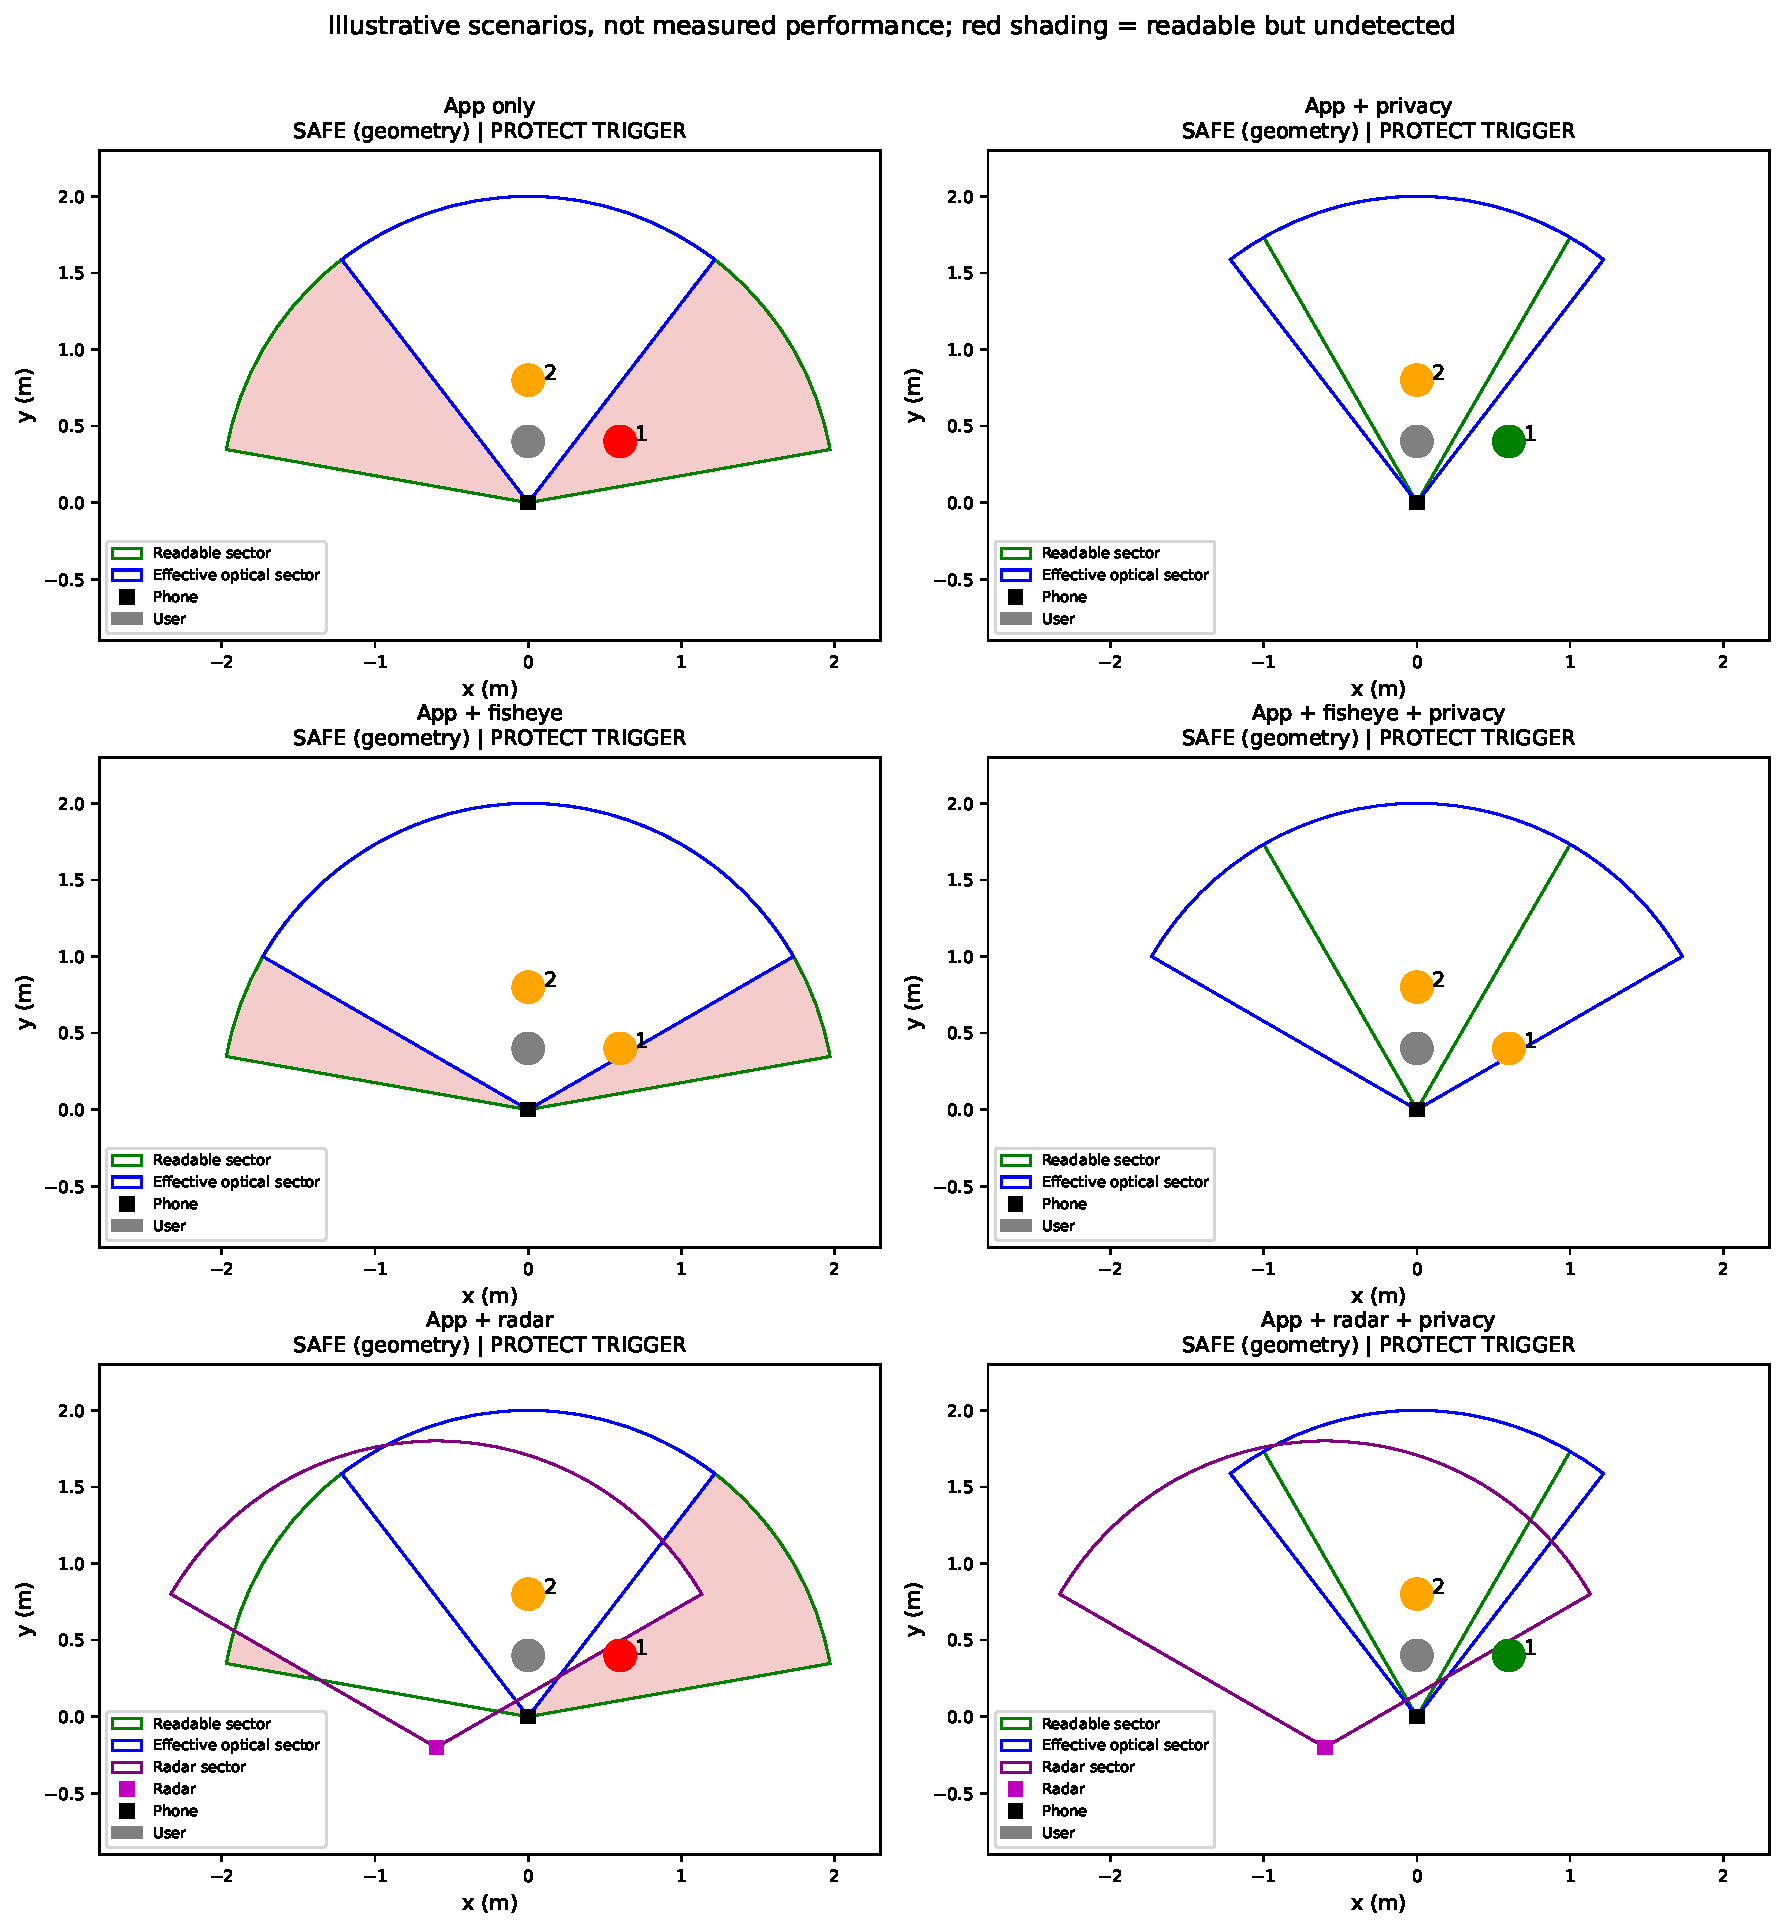
\includegraphics[width=0.96\textwidth]{figures/scenarios.pdf}
\caption{Simulator situations. Provided snapshots highlight model behavior instead of actual detector performance.}\label{fig:sim}
\end{figure*}

\section{Outcomes and Discussion}
With aligned 75-degree camera and 60-degree readable sectors, the best angular blind width is zero at each given plane distance. This is a feature of the imagined industries. It is not a zero false-negative outcome and does not fix a hidden observer on or around the screen's normalcy. The provided phone/filter combo is still the main setup to test physically.

Though it cannot remove the difference between the expected 160-degree unfiltered readable sector and narrower effective sensing, a 120-degree effective fisheye sector increases angular coverage. Including the filter can help one to leave common optical blockage and create perfect angular containment. Though its practical utility relies on accurate counting of both owner and observer, offset radar can cover areas outside the optical sector.

\begin{table}[t]\caption{Qualitative comparison; all benefits are conditional, not empirical rankings.}\centering\footnotesize
\begin{tabular}{@{}P{0.24\columnwidth}P{0.32\columnwidth}P{0.33\columnwidth}@{}}\toprule
Approach & Expected geometric effect & Residual cost/limitation\\\midrule
App + filter & Narrows readable region & Axial shoulder surfing; brightness and axis dependence\\
Fisheye + app & Enlarges optical sector & Edge quality, alignment, body occlusion\\
Fisheye + filter + app & Both changes & Same optical blind paths remain\\
Radar + app & Independent presence frame & No identity; missed/merged/stationary tracks\\
Radar + filter + app & Narrows readability plus auxiliary count & Desk placement and transform; count failures\\\bottomrule
\end{tabular}\end{table}

There is no recorded latency, battery consumption, false-positive/negative rate, recognition accuracy, or participant outcome comparison. AES-GCM guarantees the integrity and secrecy of sealed session bytes; the rendering gate manages present visual exposure; authentication helps to restore. These processes cannot replace one another. Scheduling variables—not upper limits on end-to-end response latency—are a camera frame throttle and radar specification.

\section{Limits and Upcoming Work}
One first restriction is lack of physical calibration. Before the paper is presented as an experimental validation, every situation should be replaced or augmented by recorded repeated experiments. The second is authentication validation: real-device tests are required for face embeddings, PIN rate limiting, tracking continuity, and the no-auto-reveal latch. The deployed addition is not proof of a confirmed identity threshold, resistance to presentation attacks, or limited rendering latency.

Other restrictions include lighting, face posture, masks, presentation attacks, camera blockage, per-device model performance, filter axis and brightness dependence, and unmodelled vertical geometry. Fisheye distortion and angle detection limits call for calibration following mounting. Radar adds equipment, communication failure modes, coordinate registration, and identification ambiguity. A nominal sector cannot be used to infer static-person and occlusion performance just by itself. A three-target module isn't a limitless people counter.

Future research should assess $B$ and $B_{\rm policy}$ under the same configuration, log rendering exposure times, contrast held-out recognition thresholds, and define fake locks with nearby non-observers. Participants should agree to face enrollment and utilize synthetic sensitive material. Though any stored templates call for a recorded removal and secure-storage policy, raw biometric images need not be kept. This article presents no recruited human-subject study.

\section{Final Thought}
The readable-but-undetected area gives a common goal for an adaptive privacy program, a filter, more optics, and auxiliary radar. Scenario computations first help to test the protector-plus-app setup: its readable sector fit within the estimated camera coverage. Wider optics and offset radar target different remaining areas; body occlusion and count-policy failures still exist. The source inspection, clear parameter provenance, independent simulation, and calibration process provide a repeat basis for empirical validation free from assumptions given as measurements.

\bibliographystyle{IEEEtran}
\bibliography{references}
\end{document}
